\section{Introduction to Embedded Linux}

\begin{frame}{Simplified Linux system architecture}
  \begin{center}
    \includegraphics[height=0.8\textheight]{slides/buildroot-introduction/linux-system-architecture.pdf}
  \end{center}
\end{frame}

\begin{frame}{Overall Linux boot sequence}
  \begin{center}
    \includegraphics[height=0.8\textheight]{slides/buildroot-introduction/overall-boot-sequence.pdf}
  \end{center}
\end{frame}

\begin{frame}{Embedded Linux work}
  \begin{itemize}
  \item {\bf BSP work}: porting the bootloader and Linux kernel,
    developping Linux device drivers.
  \item {\bf system integration work}: assembling all the userspace
    components needed for the system, configure them, develop the
    upgrade and recovery mechanisms, etc.
  \item {\bf application development}: write the company-specific
    applications and libraries.
  \end{itemize}
\end{frame}

\begin{frame}{Complexity of userspace integration}
  \begin{center}
    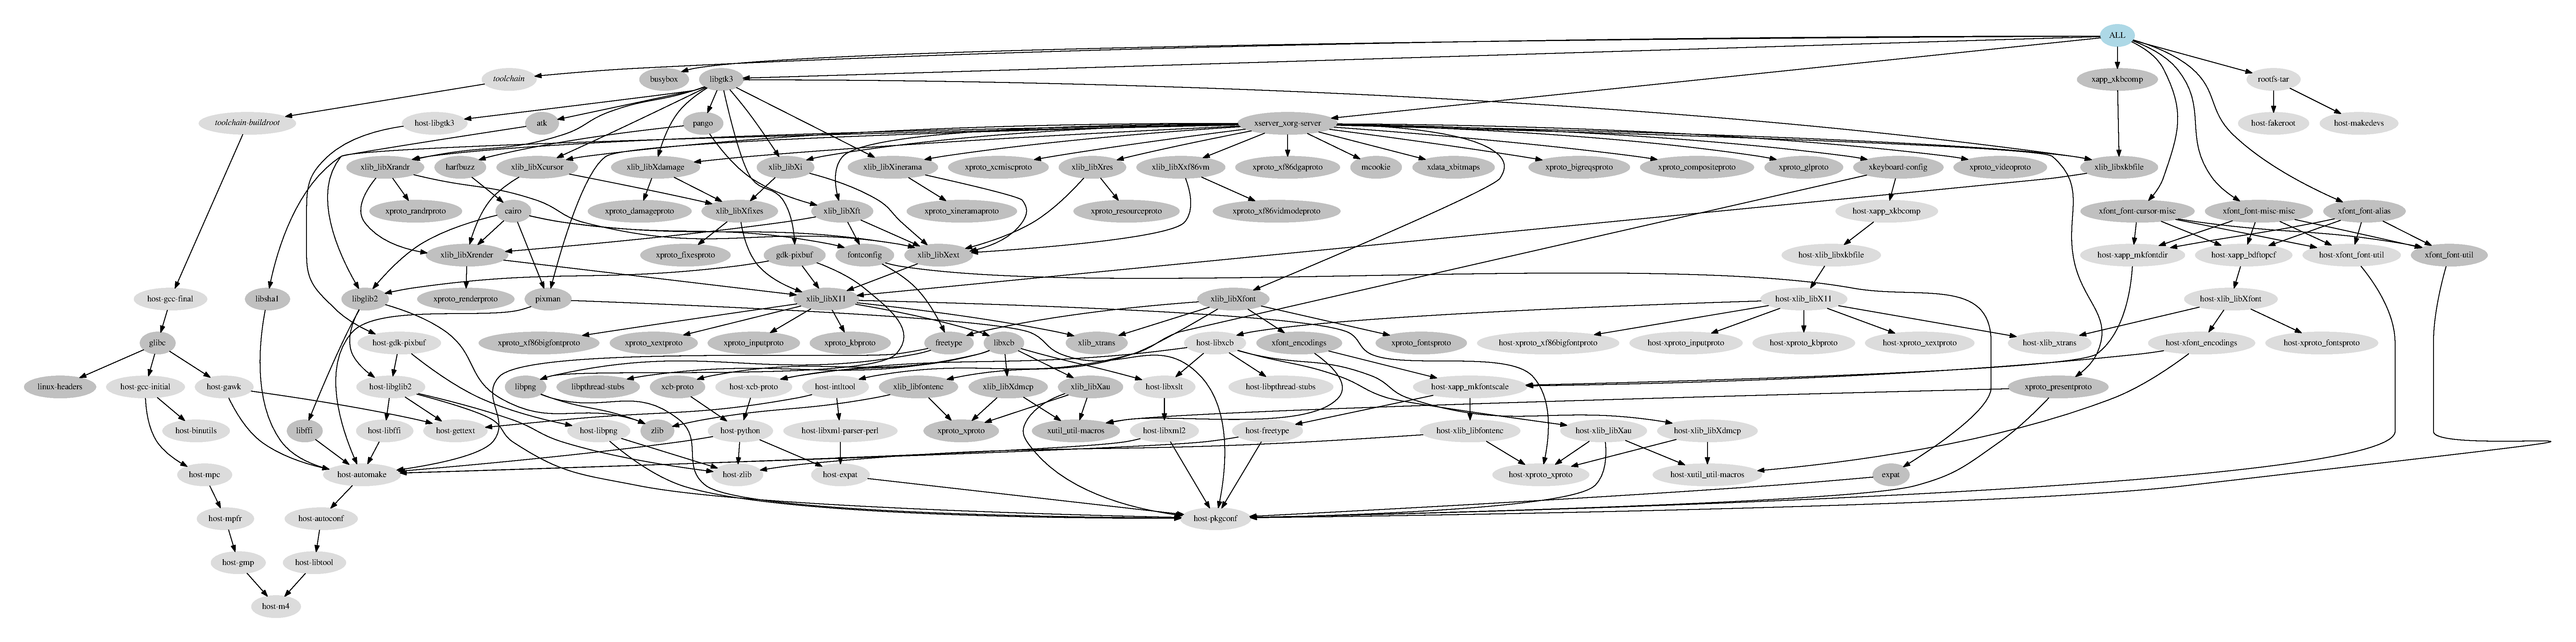
\includegraphics[width=\textwidth]{slides/buildroot-introduction/graph-depends.pdf}
  \end{center}
\end{frame}

\begin{frame}{System integration: several possibilities}
  \footnotesize
  \begin{tabularx}{11cm}{|X|X|X|}
    \hline
    & {\bf Pros} & {\bf Cons} \\
    \hline
    {\bf Building everything manually} &
    Full flexibility \newline
    Learning experience &
    Dependency hell \newline
    Need to understand a lot of details \newline
    Version compatibility \newline
    Lack of reproducitibility \\
    \hline
    {\bf Binary distribution} \newline Debian, Ubuntu, Fedora, etc.
    &
    Easy to create and extend
    &
    Hard to customize \newline
    Hard to optimize \newline
    No way to rebuild the full system from source \newline
    Large system \newline
    Usually slow boot \\
    \hline
    {\bf Build systems} \newline Buildroot, Yocto, PTXdist, etc.
    &
    Nearly full flexibility \newline
    Built from source: customization and optimization are easy \newline
    Fully reproducible
    &
    Not as easy as a binary distribution \\
    \hline
  \end{tabularx}
\end{frame}

\section{Introduction to Buildroot}

\setuplabframe
{Basic Buildroot usage}
{
  \begin{itemize}
  \item Getting and setting up Buildroot
  \item Configuring and building a basic system with Buildroot
  \item Running the system on a hardware platform and in QEMU
  \end{itemize}
}
